\chapter{Arquitetura de Software}


%Definições - principais (i.e Garlan and Shaw; Krutchen; IEEE)
%Conceitos fundamentais (comuns na literatura)
%Atributos de qualidade
%Decisões arquiteturais
%Papéis
%Visões arquiteturais
%Estilos arquiteturais

%Contexto
O desenvolvimento de um sistema de software não é uma tarefa simples por conta da complexidade envolvida no processo. Além de lidar com a complexidade inerente ao problema a ser resolvido, devemos nos preocupar em como o software resolve esse mesmo problema. Por esse motivo muitos softwares fracassam, seja por custar muito acima do orçamento, estarem imcompletos ou não solucionarem os problemas como deveriam. Assim um software além de resolver o problema, deve resolvê-lo da forma esperada, satisfazendo atributos de qualidade \cite{germoglio2010fundamentos}.

%Contexto
Conforme a complexidade dos softwares aumentam surgem adversidades. Os problemas de design vão além de algorítmos e estruturas de dados, onde a especificação da estrutura geral do sistema surge como um novo obstáculo \cite{garlan1993introduction}. Visando amenizar problemas como esse, a arquitetura de software tem recebido grande atenção  desde a década passada, já que ela tem auxiliado na obtenção de ótimos resultados quanto ao atendimento de atributos de qualidade \cite{tese_prof_fabricio}. 

Neste capítulo serão apresentados aspectos da arquitetura, relevantes durante a evolução de um sistema de software. Na seção 4.1 são apresentados os principais conceitos sobre arquitetura do ponto de vista da engenharia de software. Já a seção 4.2 expõe elementos da arquitetura do Ruby on Rails, framework utilizado para o desenvolvimento da plataforma Mezuro.

\section{Arquitetura na Engenharia de Software}

%Definição
Desde a primeira referência em um relatório técnico intitulado Software Engineering Tecnhiques \cite{buxton1970software}, na década de 1970, diversos autores buscaram definir o termo arquitetura de software de software. Abaixo se encontra uma das definições de autores que se destacaram área.

Baseados no trabalho de Mary Shaw e David Garlan \cite{shaw1996software}, Philippe Kruchten, Grady Booch, Kurt Bittner, e Rich Reitman construíram a seguinte definição para Arquitetura de software:

 “Arquitetura de Software engloba o conjunto de decisões significativas sobre a organização de um sistema de software incluindo: i) seleção de elementos estruturais e suas interfaces pelos quais um sistema é composto; ii) comportamento como especificado em colaboração entre esses elementos; iii) composição dos elementos estruturais e comportamentais dentro de um subsistema maior; iv) um estilo arquitetural que orienta essa organização. Arquitetura de Software também envolve funcionalidade, usabilidade, flexibilidade, desempenho, reuso, compreensibilidade, restrições econômicas e tecnológicas, vantagens e desvantagens, além de preocupações estéticas.”

%Motivação e Definição da ISO 1471
Essa é uma, entre diversas, definições que surgiram desde o início dos estudos relacionados a arquitetura de software. Com tantas definições é perceptível uma falta de consenso entre os autores, tanto do ponto de vista conceitual como a forma de representar uma arquitetura \cite{buschmann2007pattern}.  A falta de conformidade foi a principal motivação para a criação da ISO/IEEE 1471-2000. Com o intuito de estabelecer um padrão sobre o que é e para que serve a arquitetura de software, esse padrão não só define o termo mas também introduz um conjunto de conceitos relacionados a arquitetura. Sua definição sobre o termo é: 

“Arquitetura é a organização fundamental de um sistema incorporada em seus componentes, seus relacionamentos com o ambiente, e os princípios que conduzem seu design e evolução.”

%Elementos básicos
Apesar da falta de concordância, há três conceitos citados por todos os autores quando se trata de arquitetura de software \cite{dias2000software}. São eles:

\begin{itemize}
\item Elementos estruturais ou de software, também chamados de módulos ou componentes, são as abstrações responsáveis por representar as entidades que implementam funcionalidades especificadas.
\item Interfaces ou relacionamentos, também chamados de conectores, são as abstrações responsáveis por representar as entidades que facilitam a comunicação entre os elementos de software.
\item Organização ou configuração que consiste na forma como os elementos de software e conectores estão organizados.
\end{itemize}

%Atributos de qualidade
Durante a especificação da arquitetura é importante prestar atenção nos relacionamentos entre seus elementos. Essas relações especificam a comunicação, o controle da informação e o comportamento do sistema. Consequentemente, essas relações impactam nos atributos de qualidade, sejam os percebidos pelos usuários, ou apenas pelos desenvolvedores \cite{germoglio2010fundamentos}.

Os atributos de qualidade são uma das principais preocupações da arquitetura. Eles representam a maneira que o sistema executará suas funcionalidades e são impostos pelos diversos envolvidos no sistema. Podem ser de três tipos:

\begin{itemize}
\item Atributos de produto ditam como o sistema irá se comportar. Exemplos clássicos são: desempenho, disponibilidade, manutenbilidade, escalabilidade, disponibilidade e portabilidade;
\item Atributos organizacionais são padrões ou regras impostas por organizações envolvidas para satisfazer determinados requisitos. 
\item Atributos externos são leis impostas sobre softwares ou requisitos de interoperabilidade entre sistemas.
\end{itemize}

%Decisões Arquiteturais
Para satisfazer esses atributos a arquitetura não pode ter suas estruturas definidas aleatoriamente. É necessário que o arquiteto opte por alternativas, divida o sistema em elementos e defina seus relacionamentos para alcançar os atributos de qualidade desejados. Esse conjunto de decisões é conhecido por decisões arquiteturais. Uma decisão arquitetural possui basicamente três características, descrição, objetivos e fundamentação.

%Rastreabilidade

Qualquer software possui arquitetura, independente dela ser documentada ou projetada. Porém uma arquitetura apenas implementada, ou seja, arquitetura sem projeto, não fornece benefícios ou vantagens que uma arquitetura projetada e bem documentada pode oferecer. Entre os benefícios da documentação da arquitetura estão: i) arquitetura como ferramenta de comunicação entre os stakeholders do projeto; ii) um método ou modelo para a análise antecipada do sistema a ser desenvolvido; iii) ferramenta de rastreabilidade entre os requisitos e os elementos que compõem o sistema, o que é de grande relevância dada a volatilidade dos requisitos durante o processo de desenvolvimento.

Por relacionar atributos de qualidade (requisitos não-funcionais) a elementos arquiteturais as decisões auxiliam o rastreameto de requisitos.

%-----------------------parágrafos desconexos---------------------------------------%
Analisando o ciclo de desenvolvimento de software, é observado que a arquitetura é uma abordagem empregada desde as fases iniciais do processo. Neste instante o nível de abstração da arquitetura é bastante elevado, tendo o objetivo de definir e apresentar a solução computacional que será implementada, auxiliando a tomada de decisões dos stakeholders ou envolvidos no processo de desenvolvimento. Contudo, ao longo do desenvolvimento do software, a arquitetura sofre refinamentos que diminuem o nível de abstração e permitem, por exemplo, a representação dos relacionamentos entre os elementos arquiteturais e os arquivos de código fonte responsáveis por implementá-los \cite{clements2002documenting}.

%---------------------------------------------------------------------------------------%

\section{O Framework Ruby on Rails}

O Ruby on Rails é um framework open-source criado em 2003 por David Heinemeier Hansson, extraído de um software, um gerenciador de projetos conhecido como Basecamp.
Hansson lançou o Rails pela primeira vez ao público em 2004, e desde então seu desenvolvimento e utilização são cada vez maiores. Diversos programadores e empresas em todo mundo utilizam esse o Rails para construirem suas aplicações. Entre as mais conhecidas estão o Twitter, GitHub e Groupon. 

O Rails utiliza a linguagem de programação Ruby, criada no Japão em 1995 por Yukihiro "Matz" Matsumoto. A linguagem Ruby é interpretada, multiparadigma, com tipagem dinâmica e gerenciamento de memória automático. O Rails é basicamente uma biblioteca Ruby ou \textit{gem} e é construído utilizando o padrão arquitetural MVC.

A tabela abaixo contem todas as versões do Rails até sua última versão, assim como as datas de lançamento de cada uma.

\begin{table}[H]
\begin{center}
    \begin{tabular}{ | l | l |}
    \hline
    Versão & Data \\ \hline
    1.0 & 13/12/2005 \\ \hline
    1.2 & 19/01/2007 \\ \hline
    2.0 & 7/12/2007 \\ \hline
    2.1 & 01/06/2008 \\ \hline
    2.2 & 21/11/2008 \\ \hline
    2.3 & 16/03/2009 \\ \hline
    3.0 & 29/08/2010 \\ \hline
    3.1 & 31/08/2011 \\ \hline
    3.2 & 20/01/2012 \\ \hline
    4.0 & 25/06/2013 \\ \hline
    \end{tabular}
    \caption{Versões do Rails}
    \label{rails_versions}
\end{center}
\end{table}

%---------------------------------------------------------------------------------------%

\subsection{Evolução do Ruby on Rails}

O framework Rails, desde seu lançamento, sofre frequentes alterações, e com isso novas versões são lançadas constantemente. Muitos desenvolvedores enxergam essas constantes mudanças como um ponto negativo, ao passo que há incompatibilidade de algumas "gems" de uma versão para outra. Por outro lado, outros aprovam essa característica pois a cada atualização há melhora no produto, com adição de novos recursos, além de ser um incentivo para a implementação de testes, já que eles auxiliam a manter a integridade da aplicação a cada atualização.


Entre os novos recursos oferecidos pela versão 4 do rails estão:
\begin{itemize}
\item Páginas mais rápidas através da utilização de Turbolinks. Ao invés de deixar o navegador recompilar o JavaScript e CSS entre cada mudança de página, a instância da página atual é mantida, substituindo apenas o conteúdo e o título.
\item Suporte para a expiração de cache baseado em chave, que automatiza a invalidação do cache e deixa mais fácil a implementação de estruturas de cache sofisticadas.
\item Streaming de vídeo ao vivo em conexões persistentes.
\item Melhorias no ActiveRecord para aprimorar a consistência do escopo e da estrutura das queries.
\item Padrões de segurança locked-down.
\item Threads seguras por padrão e a eliminação da necessidade de configurar servidores com thread.
\end{itemize}


%---------------------------------------------------------------------------------------%

\subsection{Padrao Arquitetural MVC}

O padrão MVC começou como um framework desenvolvido por Trygve Reenskaug para a plataforma SmallTalk no final dos anos 70. Desde então ele exerce grande influencia sobre diversos frameworks que promovem interação com usuário.

O MVC visa separar a representação da informação da interação com o usuário. Para atingir esse objetivo são utilizados três papéis. O modelo (model) que representa informações do domínio, como dados da aplicação, regras de negócio, lógica e funções. A visão (view) que são saídas de representação dos dados do modelo ao usuário. Um exemplo comum de visão é uma pagína HTML contendo dados presentes no modelo. O útimo papel, o controlador (controller) é responsável por receber requisições da visão, manipula-las, utilizando dados do modelo, e atualizar a visão para satisfazer as requisições do usuário.

\graphicspath{{figuras/}}
\begin{figure}[H]
\centering
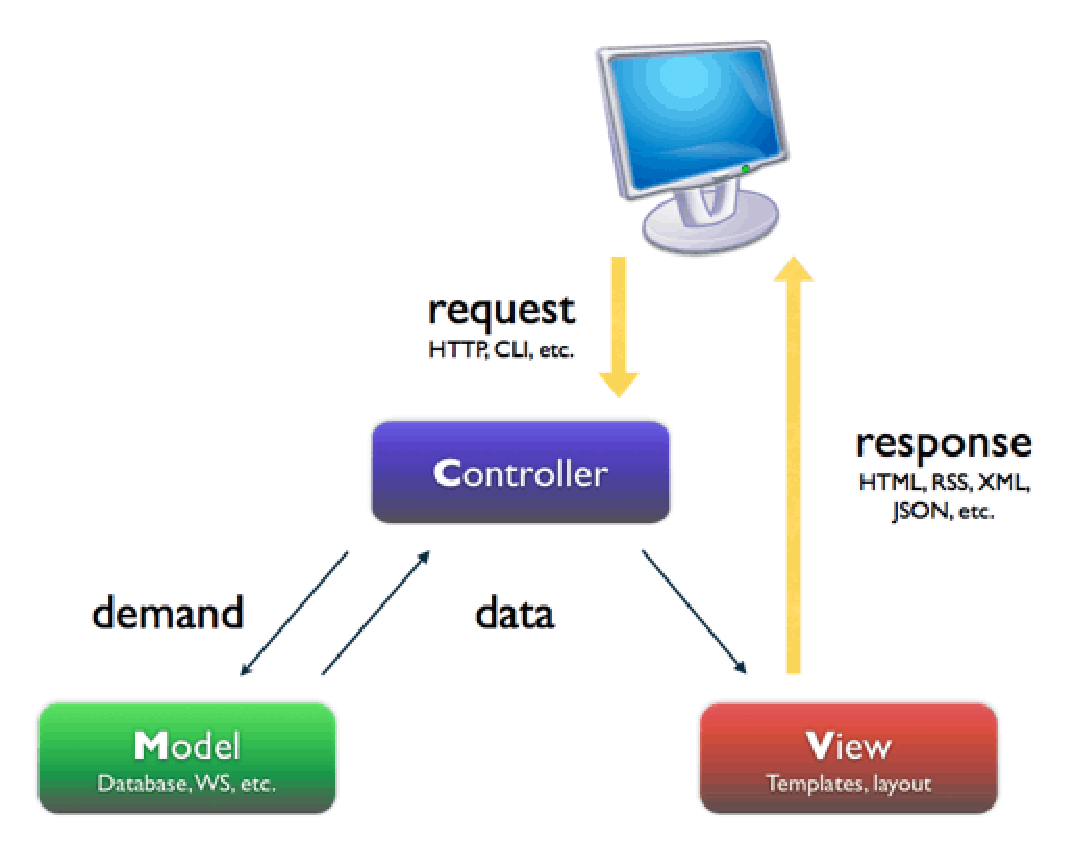
\includegraphics[width=0.5\textwidth]{mvc}
\caption{Representação do padrão MVC}
\label{mvc}
\end{figure}

O exempo abaixo ilustra um cenário de execução de uma funcionalidade com o padrão MVC.

\begin{mdframed}[frametitle={Exemplo},roundcorner=5pt, backgroundcolor=lightgray]
Um usuário navega em um site de vendas de veículos. Ao pressionar o botão para visualizar determinado veículo, o navegador carrega a página de detalhes e a devolve ao usuário. Esse processo começa quando na VIEW o usuário pressiona o botão de visualização. A URL gerada é processada por um método da CONTROLLER de veículos. Esse método solicita ao MODEL o veículo correspondente a URL, então a VIEW é renderizada com os dados do veículo correspondente, obtidos pela CONTROLLER.
\end{mdframed}

%---------------------------------------------------------------------------------------%

\subsection{Arquiterura do Rails}

Entre os elementos da arquitetura de software, há elementos estáticos e dinâmicos. Elementos estáticos definem as partes de um sistema e sua organização. Entre elementos estáticos estão: i) elementos de software; ii) elementos de dados; iii) elementos de hardware. 

As características do Rails estão distribuídas entre os seguintes elementos, ou componentes:

\begin{itemize}
\item Action Mailer
\item Action Pack
 \begin{itemize}
 \item Action Controller
 \item Action Dispactcher
 \item Action View
 \end{itemize}
\item Active Model
\item Active Record
\item Active Resource
\item Active Support
\end{itemize}

Os relacionamentos entre os elementos também estão inclusos, e também compõem o aspecto estático da arquitetura do sistema \cite{germoglio2010fundamentos}. A figura abaixo representa os elementos estáticos da arquitetura do Rails.

\graphicspath{{figuras/}}
\begin{figure}[H]
\centering
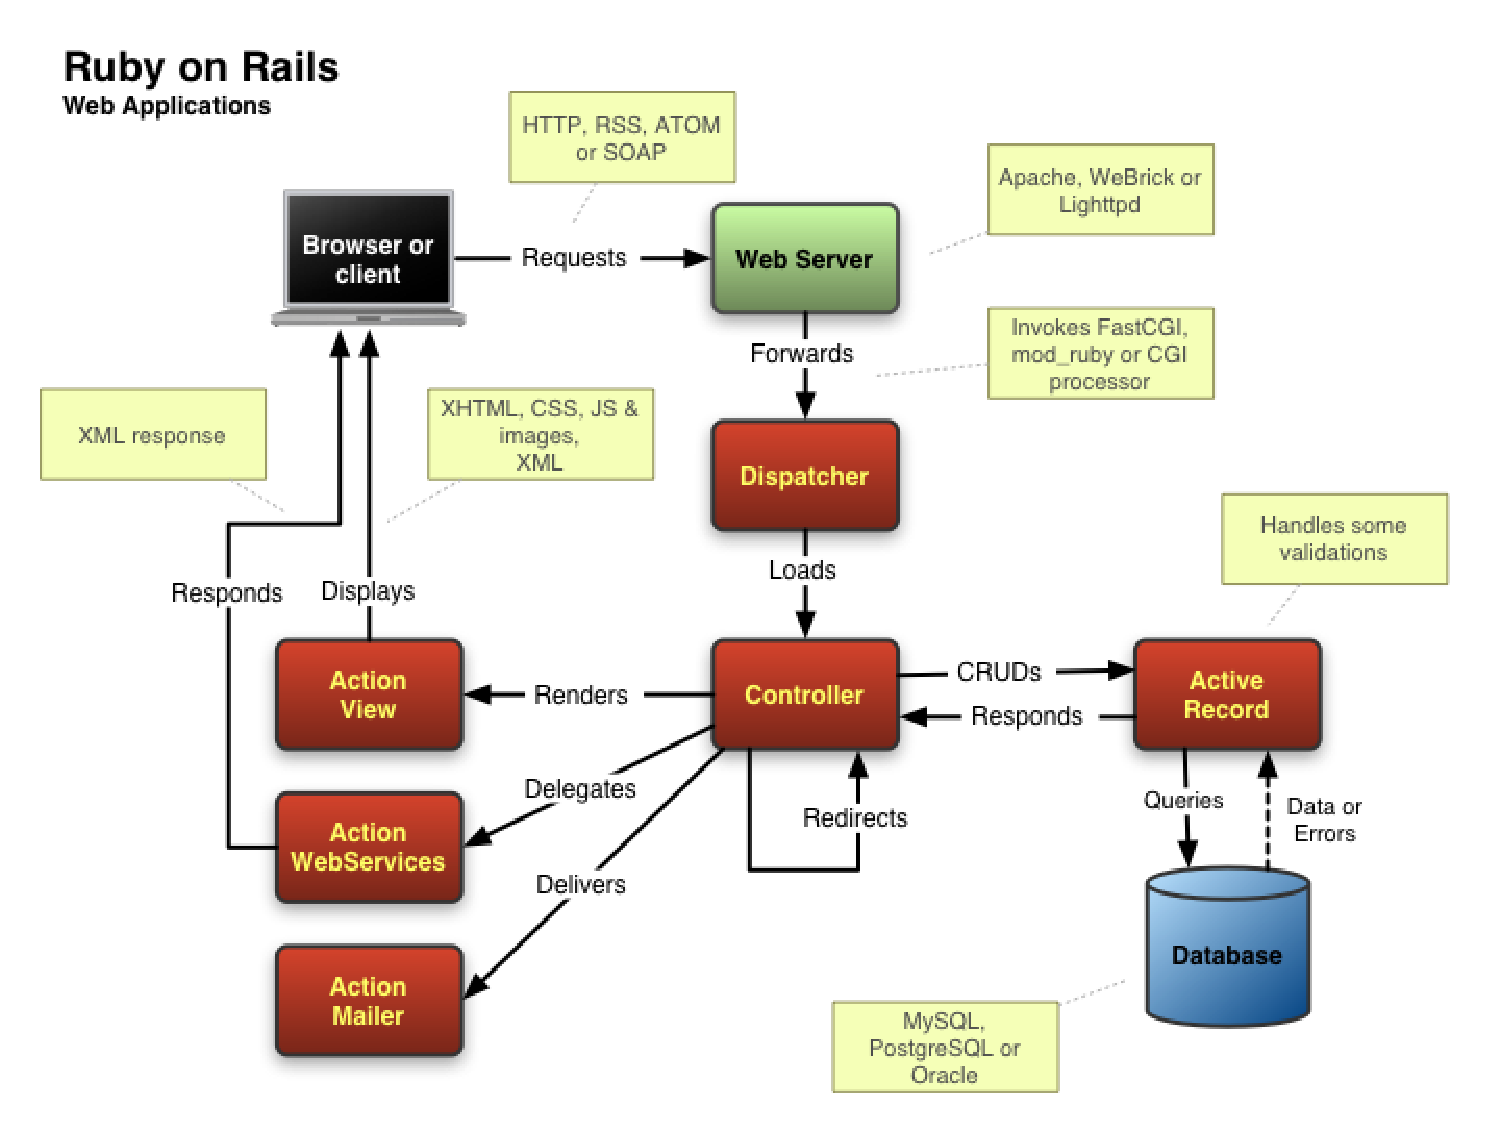
\includegraphics[width=0.7\textwidth]{rails-overview}
\caption{Interação entre os componentes do Rails. Extraído  de \cite{mejia2011rails}}
\label{rails-architecture}
\end{figure}

Já os elementos dinâmicos definem o comportamento do sistema e representa o sistema em execução. Nele estão incluídos processos, protocolos, módulos e classes que realizam comportamento.

\subsection{Plugins no Ruby on Rails}